\chapter{Experience}
\section{Wizard of Oz background}
\subsection{Definition and relevance}
The experiment is based on the "Wizard of Oz" concept of human-robot interaction. In reality, the QT-robot is not able to hear the participants or make autonomous decisions in the "Neither Yes nor No" game. Instead, we, as operators, manually controlled the course of the game and the robot's responses.

As participants interacted with the robot, we stood behind the scenes and pressed buttons to move the robot on to the next question. In addition, we also determined whether the participant's answer was "yes" or "no" by pressing separate buttons for each response. This enabled us to provide an appropriate response from the robot, saying "yes" or "no" to indicate whether the participant had lost or not.

The aim of this approach was to simulate a realistic interaction between the participants and the robot, making them believe that the robot was actually capable of understanding their responses and making decisions accordingly. Using the concept of the "Wizard of Oz", we were able to observe participants' reactions and behaviors in the face of this apparently autonomous interaction with the robot.\\
\subsection{Implementation in the VR experience}
It was easier to guarantee the context of the Wizard of Oz in VR, as the subject is fully immersed in the virtual scene. The Oculus headset works with two joysticks (one for each hand), both of which have buttons for interacting with the scene. The right joystick, held by the subject, allows him or her to launch the dialog when ready, while the left joystick allows the experimenter to skip answers or launch the end dialog if the subject has said "yes" or "no". This stratagem allows the subject to be immersed in the experiment without being aware of the "Wizard of Oz" context.
\\
\begin{figure}[!h]
\centering
\includegraphics[height=7cm]{Figures/Oz_VR.jpeg}
\caption{Control distribution system in VR}
\end{figure}\\

\subsection{Integration with robot physics experience}

To set up the "Wizard of Oz" context in the physics experiment, it was necessary to use trickery so that the participants didn't realize that the experimenter was playing the questions. Indeed, it was necessary to use a keyboard to launch the dialogue, switch from one question to another, and trigger a specific message when one of the participants used the words "yes" or "no". To divert the participants' attention and prevent them from realizing that everything was being done manually by the person to their right, the robot was positioned opposite the keyboard and the screen displaying the robot's script.

In addition, the window displaying the script was reduced to its minimum size on the screen, ensuring that subjects did not notice it. This configuration helps create the illusion of autonomous interaction between participants and the robot, reinforcing immersion in the experience.
\begin{figure}[!h]
\centering
\includegraphics[height=7cm]{Figures/magicien3.jpg}
\caption{Robot control system}
\end{figure}\\

\section{The process}
\hspace{\parindent} In order to provide the best possible answer to the question raised by the subject, we carried out an experiment to study human-robot interaction using the QT-robot in a game of "Neither yes nor no". The main aim of the experiment was to assess the impact of the robot's embodiment on interaction and engagement.\\
\\
We organized the experiment in two distinct stages. The first stage was conducted with students from our faculty, while the second stage took place in a home for all, in collaboration with a tutoring association for children from a background where most of them had never experienced virtual reality (VR) or even had the opportunity to see a robot like QT-robot. The subjects were divided into two groups, one for the robot experience and the other for the VR experience.\\
\\
After accepting the conditions of the experiment and processing the results, the first group of participants were invited to interact with the QT-robot in a game of "Neither Yes nor No". The aim was for participants to hold a conversation with the robot without uttering the words "yes" or "no". The robot was programmed to ask a series of questions and engage the participants in discussion, encouraging them to answer without using the forbidden words. If a participant managed to keep the conversation going without saying "yes" or "no" for a predetermined length of time, he or she was deemed the winner. Winners received rewards in the form of a sweet and a cake, while losers went home empty-handed.\\
\\
The second group was invited to reproduce the same "Neither Yes nor No" game, but this time using virtual reality (VR). Participants wore a VR headset that enabled them to view and interact with the QT-robot virtually. In this way, we were able to observe the differences in feel and engagement between physical interaction with the robot and virtual interaction with its VR representation.
\\
At the end of each experiment, participants were invited to complete a questionnaire specially designed for this study. They could access it by scanning the QR code provided using their phone for adults, and by filling in the paper questionnaire for children. The purpose of the questionnaire was to gather their impressions and feelings about their experience with the robot or the VR representation. The questions on the questionnaire were adapted for children to ensure that they were easy to understand.\\
\\
\begin{figure}[!h]
\centering
\includegraphics[width=2\textwidth, height=0.30\textheight,keepaspectratio]{Figures/Experience_Roadmap_Resize.png}
\caption{Experience roadmap}
\end{figure}
\\
Analysis of the responses obtained from the questionnaires will enable us to compare the differences in feeling between the two experiences, and to assess the impact of embodiment on human-robot interaction.\\

\section{The participants}

For the experiment, our professor gave us permission to promote it to the faculty students. During a project management course, we had the opportunity to invite them to participate at a later date. We also promoted the experiment on our university's Discord server. The experiment took place directly on the faculty campus. The participants were mainly students between the ages of 18 and 26, from a wide range of courses. Thanks to the Discord broadcast, we also attracted participation from students of other backgrounds and ages.\\
\\

\begin{figure}[htp]
    \centering
    \begin{minipage}[c]{0.5\textwidth}
        \centering
        \includegraphics[width=1.0\textwidth, height=0.3\textheight,keepaspectratio]{Figures/ryan.jpg}
        \caption{Physical adult experience}
    \end{minipage}%
    \begin{minipage}[c]{0.5\textwidth}
        \centering
        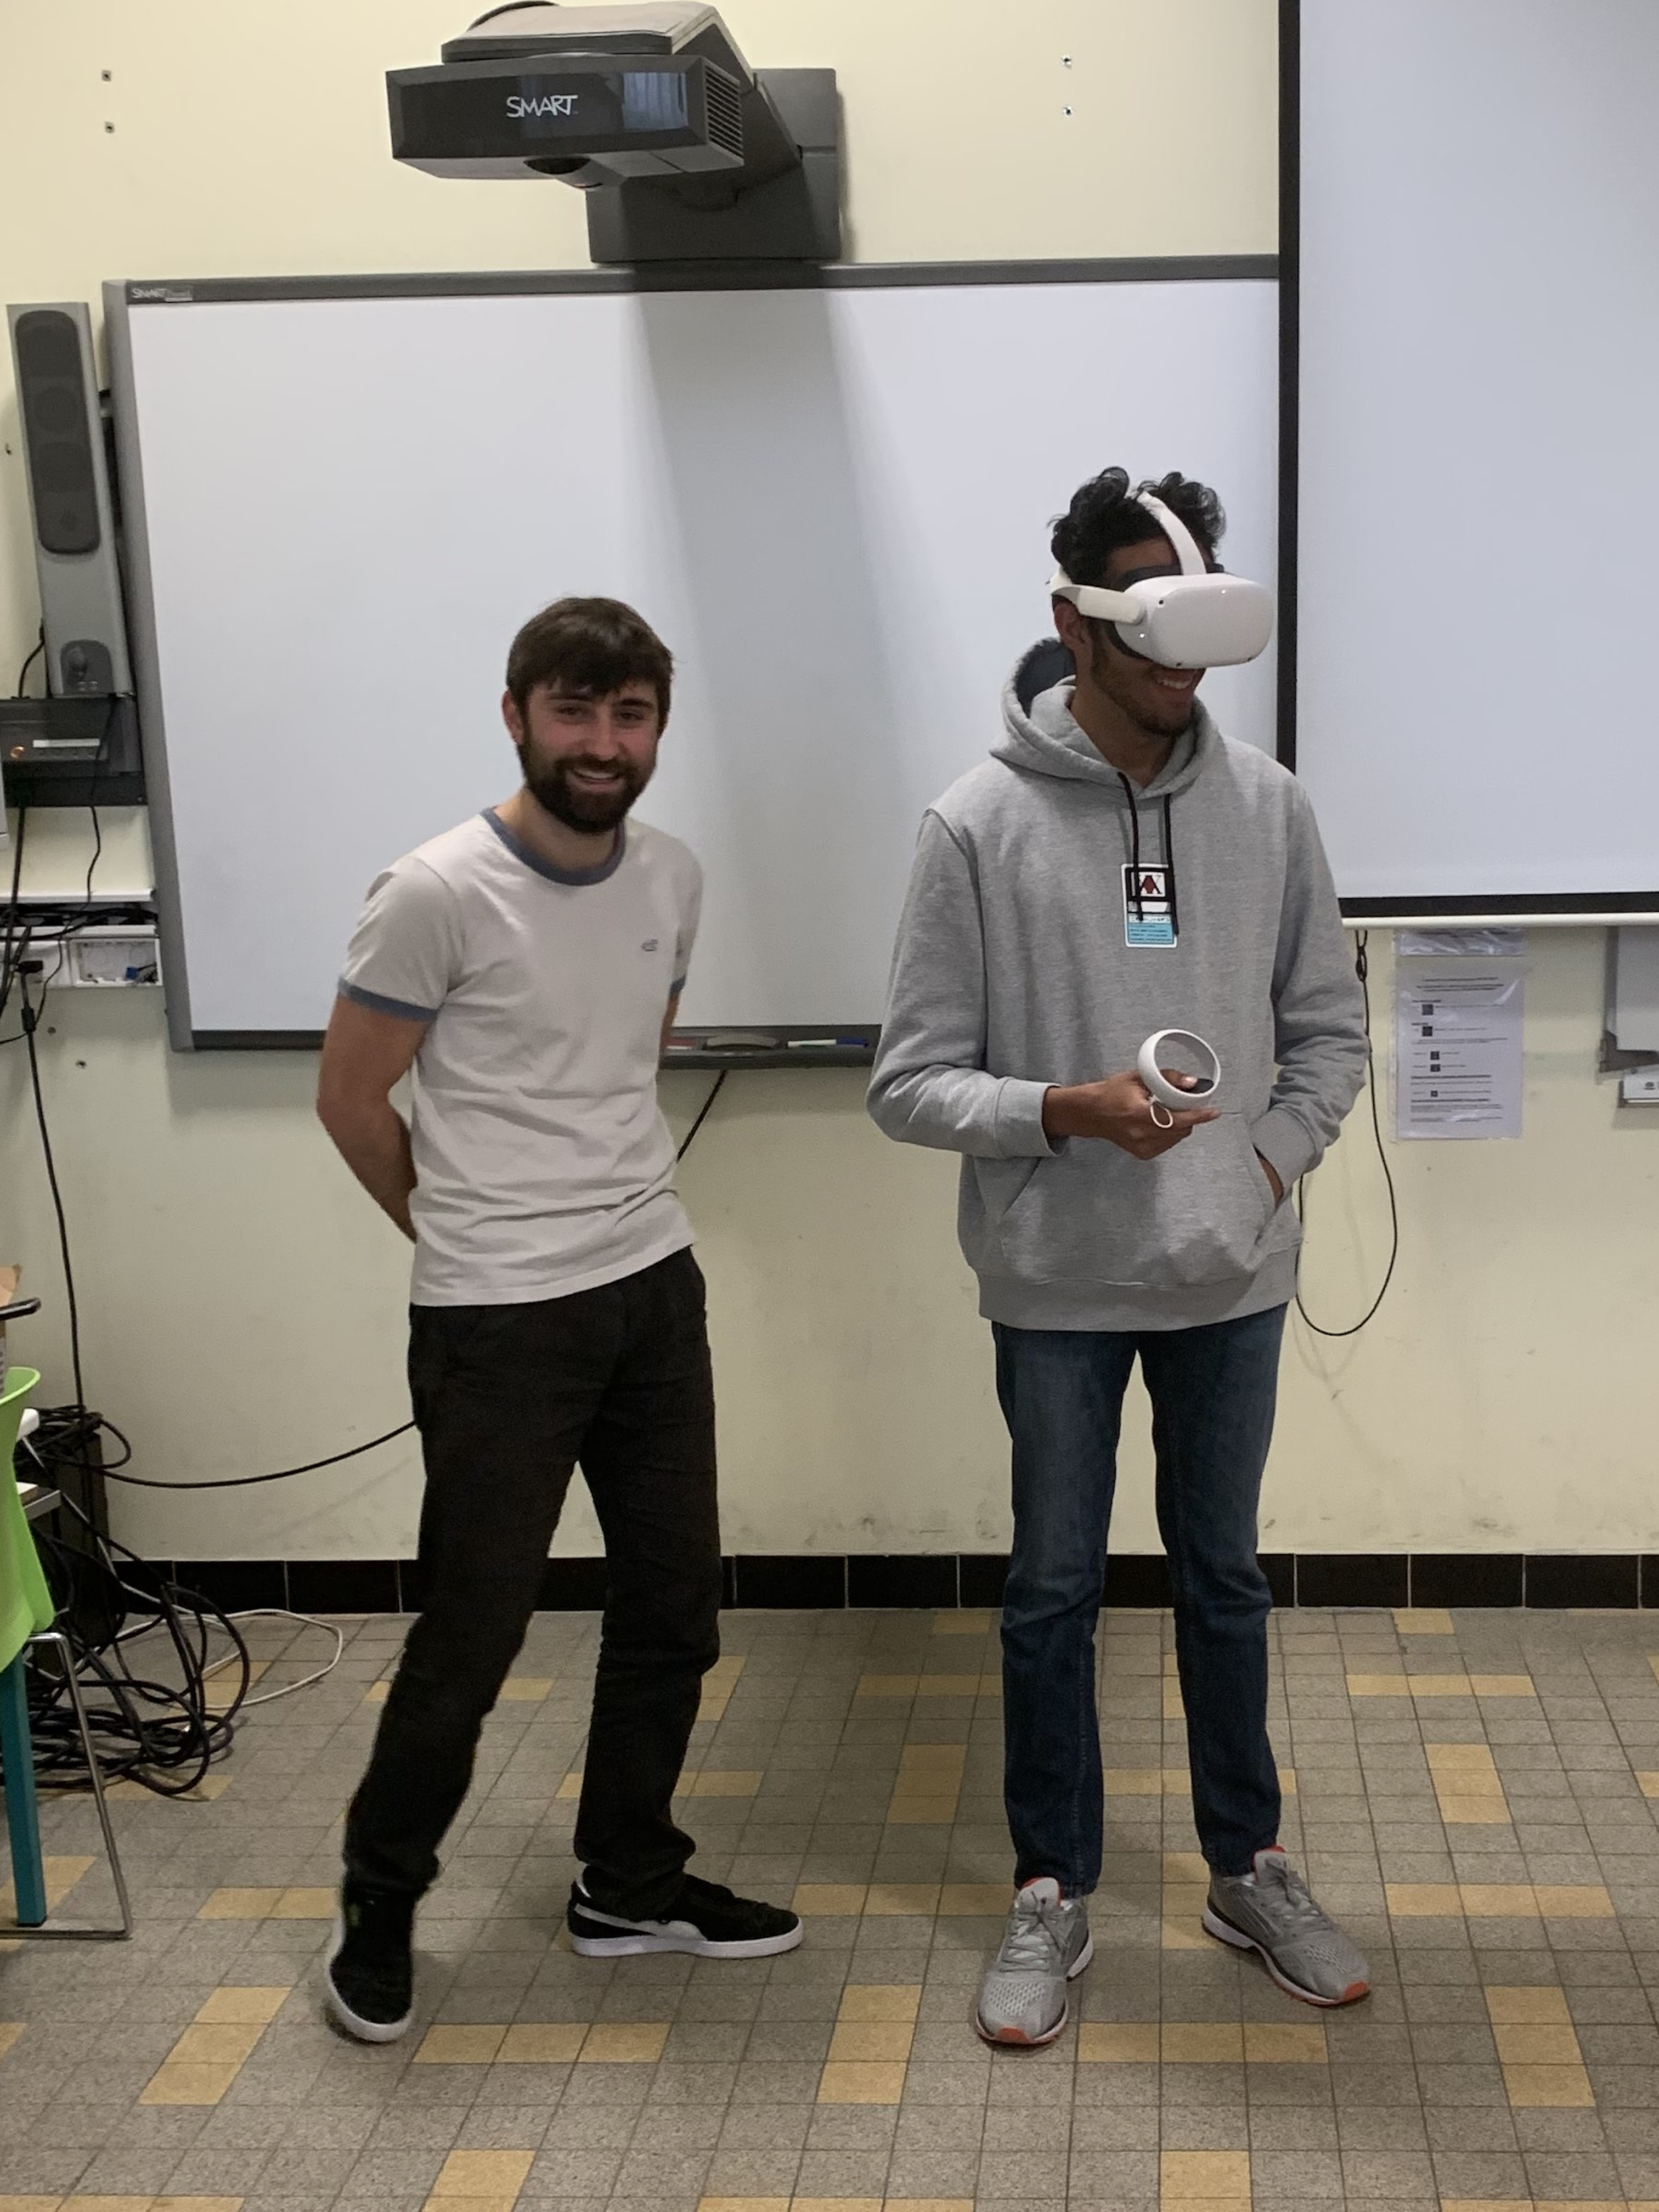
\includegraphics[width=1.0\textwidth, height=0.3\textheight,keepaspectratio]{Figures/Adulte_VR.jpg}
        \caption{Adult VR Experience}
    \end{minipage}
\end{figure}
\newpage
For the experiment with the children, knowing that one of the people in our group is a member of a children's tutoring association, we obtained permission from her tutor to carry out and present the experiment to the children of this association. We took the QT-robot, VR headset and candy to the children's home. There, we were able to connect the QT-robot to a screen and launch the "Neither Yes nor No" game. The children taking part in the experiment were aged between 9 and 15, and generally had no experience of robots or virtual reality. As the children didn't have telephones, we prepared printed questionnaire sheets on which they answered the questions.\\
\begin{figure}[htp]
    \centering
    \begin{minipage}[c]{0.5\textwidth}
        \centering
        \includegraphics[width=1.0\textwidth, height=0.3\textheight,keepaspectratio]
        {Figures/ryma.jpg}
        \caption{Physical child experience}
    \end{minipage}%
    \begin{minipage}[c]{0.5\textwidth}
        \centering
        \includegraphics[width=4\textwidth, height=0.3\textheight,keepaspectratio]{Figures/yasmina.jpg}
        \caption{Children's VR experience}
    \end{minipage}
\end{figure}
\\

